% !TeX TXS-program:compile = txs:///pdflatex/[--shell-escape]

\documentclass[11pt, letterpaper]{article}

\usepackage[utf8]{inputenc}
\usepackage[T1]{fontenc}
\usepackage{lmodern}
\usepackage{graphicx}
\usepackage{longtable}
\usepackage{wrapfig}
\usepackage{rotating}
\usepackage{amsmath}
\usepackage{textcomp}
\usepackage{amssymb}
\usepackage{hyperref}
\usepackage[spanish]{babel}
\usepackage[round]{natbib}
\usepackage{subcaption}

\title{\bfseries Tarea}
\author{Ángel García Báez}
\date{\today}
\setcounter{tocdepth}{4} 

\begin{document}
	% Página de presentación
	\begin{titlepage}
		\centering
		
\includegraphics[width=0.2\textwidth]{logo.png}\par
		\vspace{1cm}
		{\LARGE \bfseries Universidad Veracruzana \par}
		\vspace{1cm}
		{\Large Maestría en Inteligencia Artificial\par}
		\vspace{3cm}
		{\LARGE \bfseries Lógica difusa \par}
		\vspace{1cm}
		{\Large \bfseries Tarea 4. Problema de la calificación de videojuegos con lógica difusa programado paso a paso en MATLAB implementando el método de desfuzzificación Centro del Área. \par}
		\vfill
		{\Large \textit{Ángel García Báez}\par}
		\vfill
		{\Large Dr. Sergio Hernández Méndez \par}
		\vfill
		{\Large \today \par}
	\end{titlepage}
	
	% Página exclusiva para la tabla de contenidos
	\newpage
	\tableofcontents
	\newpage
	
% Explicación breve

\section{Introducción}

En el presente reporte se explica brevemente la propuesta del problema de calificar videojuegos en base a 3 variables (historia, jugabilidad y gráficos),se explica brevemente el proceso de implementación para la resolución del problema con salidas gaussianas, para el cual fue necesario extender el programa hecho en la tarea 3 para que procesara tres entradas distintas, junto con su respectivo aumento en la base de reglas. La salida se modelo como una gaussiana mediante el proceso de desfuzificación centro del área.

Con la finalidad de comparar que tan buena fue la implementación propia, se hace la comparativa entre los resultados obtenidos con el paquete de Fuzzy Logic de matlab y el programa implementado paso a paso en 3 escenarios distintos: caso mínimo, caso intermedio y caso máximo.


\newpage


\section{Problema 1: Calificación de videojuegos}

\subsection{Explicación del Problema}

Se tiene la duda sobre las calificaciones que se otorgan a distintos videojuegos en paginas especializadas como metacritic, puesto que hasta donde se tiene conocimiento, la nota que se muestra en la pagina es el producto de una media ponderada obtenida mediante la opinión de distintos medios pero se desconoce como es que estos afectan a la nota, puesto que juegos que son malos según los jugadores aparecen con notas medias por encima del 80 y al revés, juegos buenos y aclamados por los jugadores aparecen con notas menores a 70.

Con la finalidad de tener un acercamiento al modelado de la calificación que se les da a los videojuegos mediante un sistema de lógica difusa compuesto por 3 variables de entrada: Jugabilidad, Gráficos e Historia, modeladas mediante funciones de membresía Gaussianas tanto para las entradas como para las salidas.


\subsection{Variables y sus codificaciones}

A continuación se listan los valores de las variables lingüísticas que se
propusieron para SERVICIO, COMIDA y PROPINA como sigue:

\begin{enumerate}
	\item Jugabilidad: Mala ($\mu = 10$, $\sigma = 25$), Regular ($\mu = 60$, $\sigma = 10$) y Buena ($\mu = 80$, $\sigma = 10$).
	\begin{figure}[h]
		\centering
		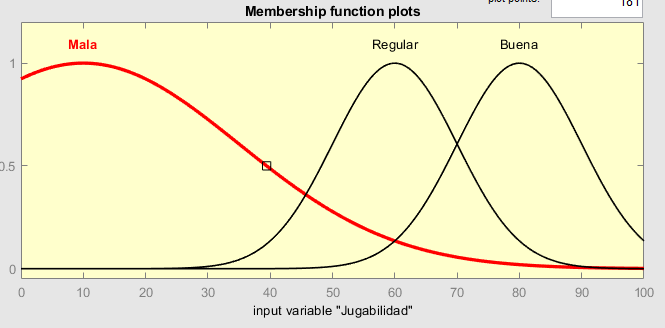
\includegraphics[width=0.8\textwidth]{IMG/P11.png}
	\end{figure}
	\newpage
	\item Gráficos: Malos ($\mu = 20$, $\sigma = 15$), Decentes ($\mu = 50$, $\sigma = 10$) y Excelentes ($\mu = 80$, $\sigma = 15$).
	\begin{figure}[h]
		\centering
		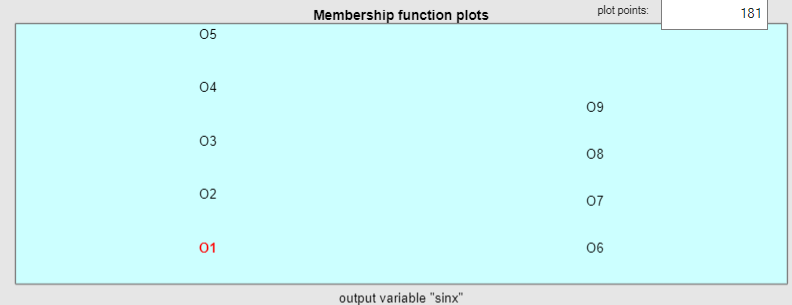
\includegraphics[width=0.8\textwidth]{IMG/P12.png}
	\end{figure}
	\item Historia: Pésima ($\mu = 20$, $\sigma = 15$), Pasable ($\mu = 60$, $\sigma = 12$) y Excelente ($\mu = 85$, $\sigma = 10$).
	\begin{figure}[h]
		\centering
		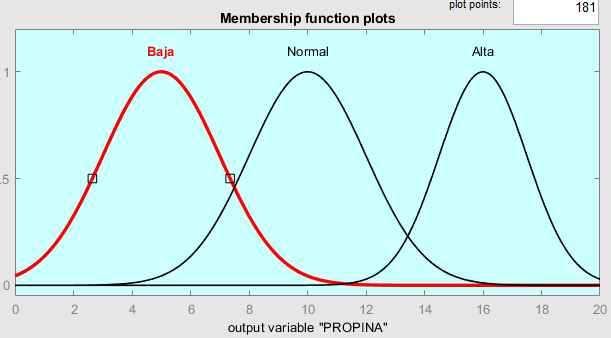
\includegraphics[width=0.8\textwidth]{IMG/P13.png}
	\end{figure}
	\newpage
	\item Calificación: Pésimo ($\mu = 20$, $\sigma = 15$), Pasable ($\mu = 55$, $\sigma = 12$) y Excelente ($\mu = 85$, $\sigma = 10$).
	\begin{figure}[h]
		\centering
		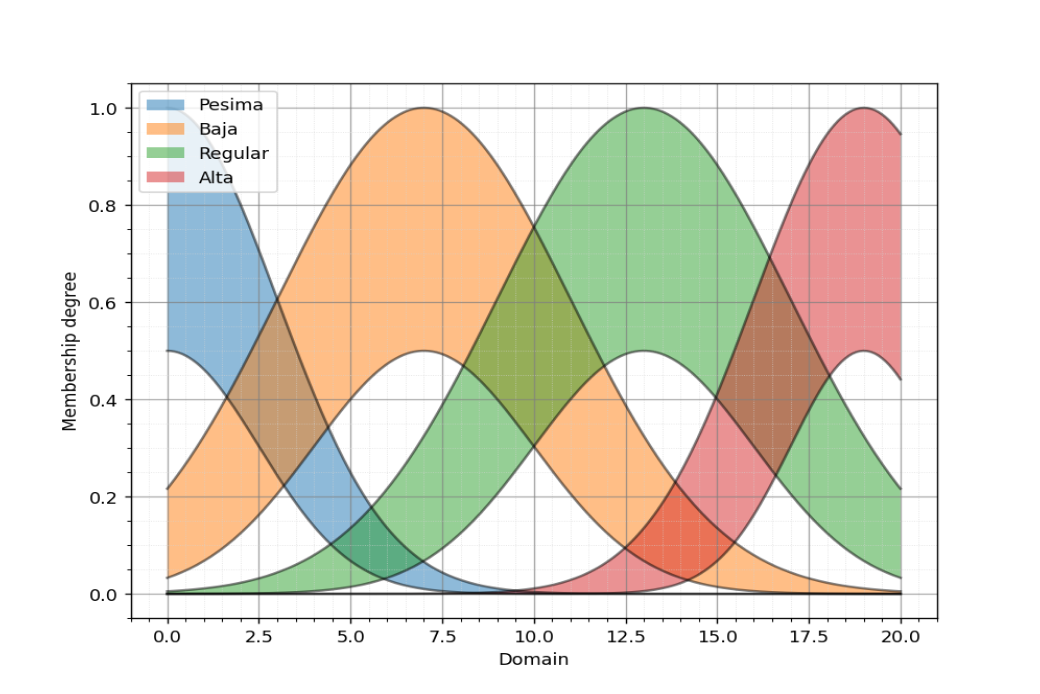
\includegraphics[width=0.8\textwidth]{IMG/P14.png}
	\end{figure}
\end{enumerate}

Todas las funciones de membresía se mantuvieron Gaussianas.

Se mantuvo el método de desfuzzificación del centroide (centro de masa) para todas las funciones con la inferencia de Mandani para los resultados obtenidos mediante el fuzzy toolbox de matlab.\\

\newpage

\subsection{Reglas de inferencia.}

A continuación se muestra la base de reglas compuesta por 27 reglas de la forma AND:

\begin{enumerate}
	\item R1: Si \textbf{JUGABILIDAD} es \textbf{\textit{MALA}} y los \textbf{GRÁFICOS} son \textbf{\textit{MALOS}} y la \textbf{HISTORIA} es \textbf{\textit{PÉSIMA}}, la \textbf{CALIFICACIÓN} es \textbf{\textit{PÉSIMA}}.
	\item R2: Si \textbf{JUGABILIDAD} es \textbf{\textit{MALA}} y los \textbf{GRÁFICOS} son \textbf{\textit{MALOS}} y la \textbf{HISTORIA} es \textbf{\textit{PASABLE}}, la \textbf{CALIFICACIÓN} es \textbf{\textit{PÉSIMA}}.
	\item R3: Si \textbf{JUGABILIDAD} es \textbf{\textit{MALA}} y los \textbf{GRÁFICOS} son \textbf{\textit{MALOS}} y la \textbf{HISTORIA} es \textbf{\textit{EXCELENTE}}, la \textbf{CALIFICACIÓN} es \textbf{\textit{PÉSIMA}}.
	\item R4: Si \textbf{JUGABILIDAD} es \textbf{\textit{MALA}} y los \textbf{GRÁFICOS} son \textbf{\textit{DECENTES}} y la \textbf{HISTORIA} es \textbf{\textit{PÉSIMA}}, la \textbf{CALIFICACIÓN} es \textbf{\textit{PÉSIMA}}.
	\item R5: Si \textbf{JUGABILIDAD} es \textbf{\textit{MALA}} y los \textbf{GRÁFICOS} son \textbf{\textit{DECENTES}} y la \textbf{HISTORIA} es \textbf{\textit{PASABLE}}, la \textbf{CALIFICACIÓN} es \textbf{\textit{PÉSIMA}}.
	\item R6: Si \textbf{JUGABILIDAD} es \textbf{\textit{MALA}} y los \textbf{GRÁFICOS} son \textbf{\textit{DECENTES}} y la \textbf{HISTORIA} es \textbf{\textit{EXCELENTE}}, la \textbf{CALIFICACIÓN} es \textbf{\textit{PASABLE}}.
	\item R7: Si \textbf{JUGABILIDAD} es \textbf{\textit{MALA}} y los \textbf{GRÁFICOS} son \textbf{\textit{EXCELENTES}} y la \textbf{HISTORIA} es \textbf{\textit{PÉSIMA}}, la \textbf{CALIFICACIÓN} es \textbf{\textit{PÉSIMA}}.
	\item R8: Si \textbf{JUGABILIDAD} es \textbf{\textit{MALA}} y los \textbf{GRÁFICOS} son \textbf{\textit{EXCELENTES}} y la \textbf{HISTORIA} es \textbf{\textit{PASABLE}}, la \textbf{CALIFICACIÓN} es \textbf{\textit{PASABLE}}.
	\item R9: Si \textbf{JUGABILIDAD} es \textbf{\textit{MALA}} y los \textbf{GRÁFICOS} son \textbf{\textit{EXCELENTES}} y la \textbf{HISTORIA} es \textbf{\textit{EXCELENTE}}, la \textbf{CALIFICACIÓN} es \textbf{\textit{PASABLE}}.
	\item R10: Si \textbf{JUGABILIDAD} es \textbf{\textit{REGULAR}} y los \textbf{GRÁFICOS} son \textbf{\textit{MALOS}} y la \textbf{HISTORIA} es \textbf{\textit{PÉSIMA}}, la \textbf{CALIFICACIÓN} es \textbf{\textit{PÉSIMA}}.
	\item R11: Si \textbf{JUGABILIDAD} es \textbf{\textit{REGULAR}} y los \textbf{GRÁFICOS} son \textbf{\textit{MALOS}} y la \textbf{HISTORIA} es \textbf{\textit{PASABLE}}, la \textbf{CALIFICACIÓN} es \textbf{\textit{PASABLE}}.
	\item R12: Si \textbf{JUGABILIDAD} es \textbf{\textit{REGULAR}} y los \textbf{GRÁFICOS} son \textbf{\textit{MALOS}} y la \textbf{HISTORIA} es \textbf{\textit{EXCELENTE}}, la \textbf{CALIFICACIÓN} es \textbf{\textit{PASABLE}}.
	\item R13: Si \textbf{JUGABILIDAD} es \textbf{\textit{REGULAR}} y los \textbf{GRÁFICOS} son \textbf{\textit{DECENTES}} y la \textbf{HISTORIA} es \textbf{\textit{PÉSIMA}}, la \textbf{CALIFICACIÓN} es \textbf{\textit{PASABLE}}.
	\item R14: Si \textbf{JUGABILIDAD} es \textbf{\textit{REGULAR}} y los \textbf{GRÁFICOS} son \textbf{\textit{DECENTES}} y la \textbf{HISTORIA} es \textbf{\textit{PASABLE}}, la \textbf{CALIFICACIÓN} es \textbf{\textit{PASABLE}}.
	\item R15: Si \textbf{JUGABILIDAD} es \textbf{\textit{REGULAR}} y los \textbf{GRÁFICOS} son \textbf{\textit{DECENTES}} y la \textbf{HISTORIA} es \textbf{\textit{EXCELENTE}}, la \textbf{CALIFICACIÓN} es \textbf{\textit{EXCELENTE}}.
	\item R16: Si \textbf{JUGABILIDAD} es \textbf{\textit{REGULAR}} y los \textbf{GRÁFICOS} son \textbf{\textit{EXCELENTES}} y la \textbf{HISTORIA} es \textbf{\textit{PÉSIMA}}, la \textbf{CALIFICACIÓN} es \textbf{\textit{PASABLE}}.
	\item R17: Si \textbf{JUGABILIDAD} es \textbf{\textit{REGULAR}} y los \textbf{GRÁFICOS} son \textbf{\textit{EXCELENTES}} y la \textbf{HISTORIA} es \textbf{\textit{PASABLE}}, la \textbf{CALIFICACIÓN} es \textbf{\textit{EXCELENTE}}.
	\item R18: Si \textbf{JUGABILIDAD} es \textbf{\textit{REGULAR}} y los \textbf{GRÁFICOS} son \textbf{\textit{EXCELENTES}} y la \textbf{HISTORIA} es \textbf{\textit{EXCELENTE}}, la \textbf{CALIFICACIÓN} es \textbf{\textit{EXCELENTE}}.
	\item R19: Si \textbf{JUGABILIDAD} es \textbf{\textit{BUENA}} y los \textbf{GRÁFICOS} son \textbf{\textit{MALOS}} y la \textbf{HISTORIA} es \textbf{\textit{PÉSIMA}}, la \textbf{CALIFICACIÓN} es \textbf{\textit{PASABLE}}.
	\item R20: Si \textbf{JUGABILIDAD} es \textbf{\textit{BUENA}} y los \textbf{GRÁFICOS} son \textbf{\textit{MALOS}} y la \textbf{HISTORIA} es \textbf{\textit{PASABLE}}, la \textbf{CALIFICACIÓN} es \textbf{\textit{PASABLE}}.
	\item R21: Si \textbf{JUGABILIDAD} es \textbf{\textit{BUENA}} y los \textbf{GRÁFICOS} son \textbf{\textit{MALOS}} y la \textbf{HISTORIA} es \textbf{\textit{EXCELENTE}}, la \textbf{CALIFICACIÓN} es \textbf{\textit{PASABLE}}.
	\item R22: Si \textbf{JUGABILIDAD} es \textbf{\textit{BUENA}} y los \textbf{GRÁFICOS} son \textbf{\textit{DECENTES}} y la \textbf{HISTORIA} es \textbf{\textit{PÉSIMA}}, la \textbf{CALIFICACIÓN} es \textbf{\textit{PASABLE}}.
	\item R23: Si \textbf{JUGABILIDAD} es \textbf{\textit{BUENA}} y los \textbf{GRÁFICOS} son \textbf{\textit{DECENTES}} y la \textbf{HISTORIA} es \textbf{\textit{PASABLE}}, la \textbf{CALIFICACIÓN} es \textbf{\textit{EXCELENTE}}.
	\item R24: Si \textbf{JUGABILIDAD} es \textbf{\textit{BUENA}} y los \textbf{GRÁFICOS} son \textbf{\textit{DECENTES}} y la \textbf{HISTORIA} es \textbf{\textit{EXCELENTE}}, la \textbf{CALIFICACIÓN} es \textbf{\textit{EXCELENTE}}.
	\item R25: Si \textbf{JUGABILIDAD} es \textbf{\textit{BUENA}} y los \textbf{GRÁFICOS} son \textbf{\textit{EXCELENTES}} y la \textbf{HISTORIA} es \textbf{\textit{PÉSIMA}}, la \textbf{CALIFICACIÓN} es \textbf{\textit{PASABLE}}.
	\item R26: Si \textbf{JUGABILIDAD} es \textbf{\textit{BUENA}} y los \textbf{GRÁFICOS} son \textbf{\textit{EXCELENTES}} y la \textbf{HISTORIA} es \textbf{\textit{PASABLE}}, la \textbf{CALIFICACIÓN} es \textbf{\textit{EXCELENTE}}.
	\item R27: Si \textbf{JUGABILIDAD} es \textbf{\textit{BUENA}} y los \textbf{GRÁFICOS} son \textbf{\textit{EXCELENTES}} y la \textbf{HISTORIA} es \textbf{\textit{EXCELENTE}}, la \textbf{CALIFICACIÓN} es \textbf{\textit{EXCELENTE}}.
\end{enumerate}

\newpage

\subsection{Gráficos del problema de las calificaciones}

La gráfica de superficie resultante del problema con entradas y salidas Gaussianas junto con la base de reglas ya mencionada toma la siguiente forma:

\begin{figure}[h]
	\centering
	\begin{subfigure}{0.42\textwidth} % Reducido de 0.45
		\centering
		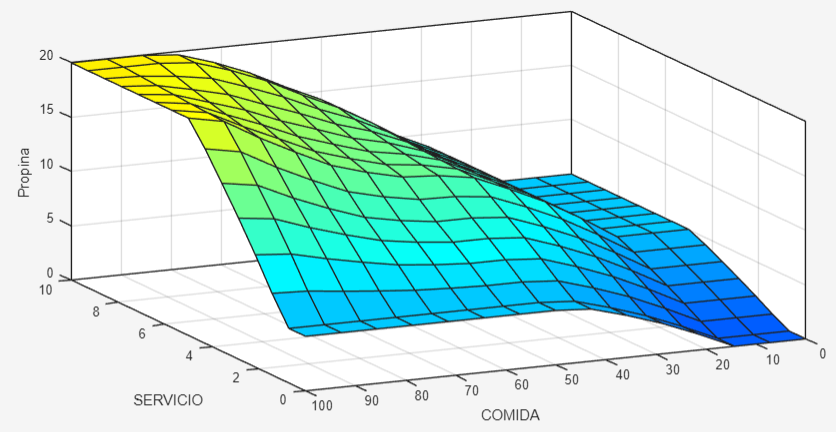
\includegraphics[width=1.3\textwidth]{IMG/P15.png}
		\label{fig:G1}
	\end{subfigure}
	\hfill
	\begin{subfigure}{0.42\textwidth} % Reducido de 0.45
		\centering
		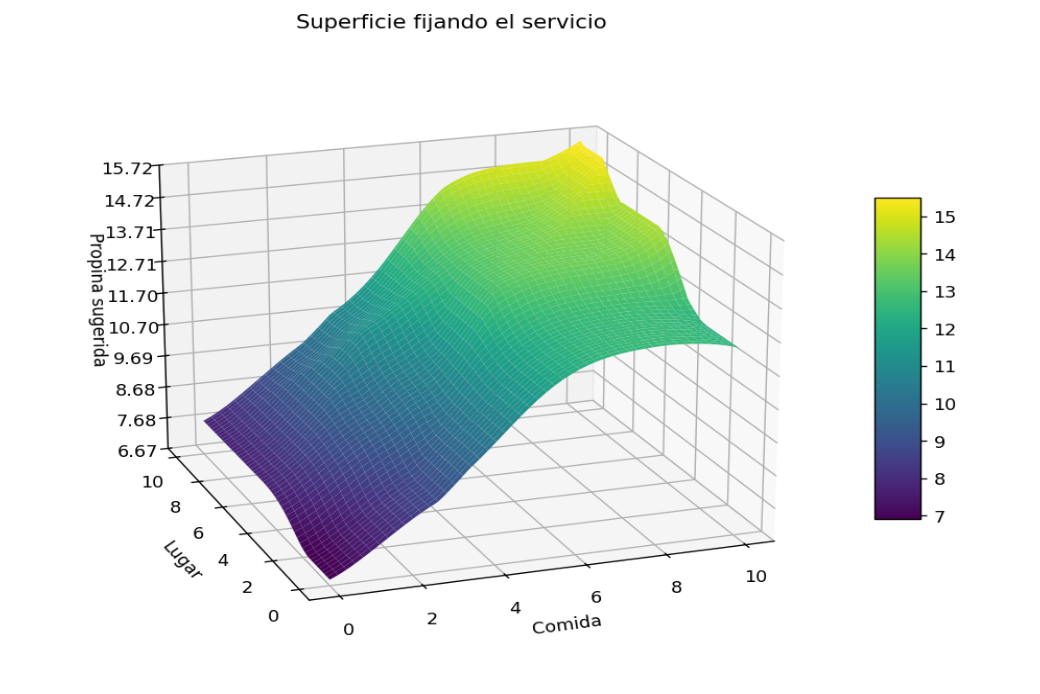
\includegraphics[width=1.2\textwidth]{IMG/P16.png}
		\label{fig:G2}
	\end{subfigure}
	\label{fig:comparacion1}
\end{figure}
\begin{figure}[h]
	\centering
	\begin{subfigure}{0.42\textwidth} % Mismo formato que arriba
		\centering
		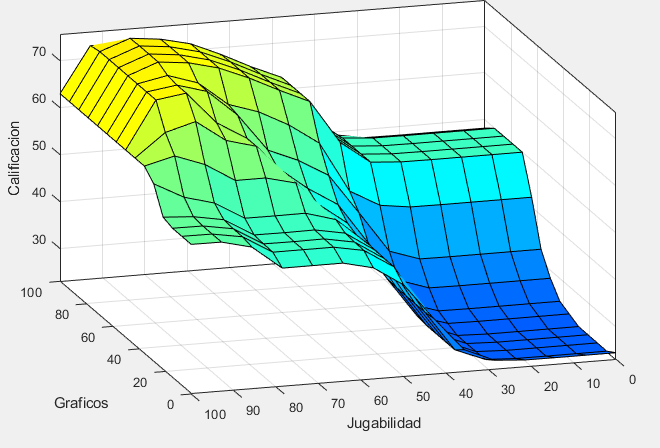
\includegraphics[width=1.3\textwidth]{IMG/P17.png}
		\label{fig:G31}
	\end{subfigure}
	\hfill
	\begin{subfigure}{0.42\textwidth} % Mismo formato que arriba
		\centering
		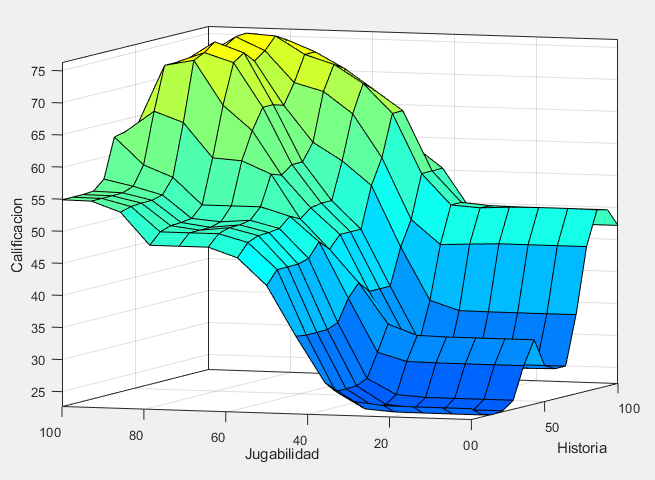
\includegraphics[width=1.2\textwidth]{IMG/P18.png}
		\label{fig:G41}
	\end{subfigure}
	\label{fig:comparacion21}
\end{figure}

Dado que la gráfica esta compuesta por 3 variables,. es necesario visualizarla por pares de variables para poder hacerse una idea de su comportamiento.

Se observa como presenta un comportamiento gradualmente descendiente relativamente suave, pero existe una zona donde cae abruptamente, puede servir esto como aviso de que las reglas o los rangos de las variables necesitan ser re-ajustados.

\newpage

\subsection{Implementación del problema de la calificación de videojuegos con desfuzzificación del centro de sumas paso a paso}

Como se menciono en un inicio, el principal objetivo de esta actividad es implementar uno mismo el sistema de lógica difusa para comparar los resultados con respecto de los mostrados por el fuzzy toolbox de matlab.\\

El primer paso  identificar las variables de discurso SERVICIO, COMIDA y PROPINA para inicializarlas en 0.\\

Con referencia a lo explicado en el libro de \cite{Cisneros2004}, se implemento la función de membresía Gaussiana tal y como la define a continuación:

\[
f(x, \mu, \sigma) = e^{\left( \frac{(x - \mu)^2}{2\sigma^2} \right)}
\]

Posteriormente, se definieron los rangos de cada una de las funciones de membresía, dado que solo se usan funciones gaussianas, se dejaron los rangos tal cual se había presentado anteriormente:

\begin{enumerate}
\item Jugabilidad: Mala ($\mu = 10$, $\sigma = 25$), Regular ($\mu = 60$, $\sigma = 10$) y Buena ($\mu = 80$, $\sigma = 10$).
\item Gráficos: Malos ($\mu = 20$, $\sigma = 15$), Decentes ($\mu = 50$, $\sigma = 10$) y Excelentes ($\mu = 80$, $\sigma = 15$).
\item Historia: Pésima ($\mu = 20$, $\sigma = 15$), Pasable ($\mu = 60$, $\sigma = 12$) y Excelente ($\mu = 85$, $\sigma = 10$).
\item Calificación: Pésimo ($\mu = 20$, $\sigma = 15$), Pasable ($\mu = 55$, $\sigma = 12$) y Excelente ($\mu = 85$, $\sigma = 10$).
\end{enumerate} 


Siguiendo con el proceso, fueron implementadas cada una las 12 reglas que ya se mostraron previamente, haciendo uso de la operación de conjuntos difusos $AND$, para esto, la activación de las reglas del sistema se determinan de la siguiente forma:

\[
\text{Activación de regla}  = \min( \mu_A(X), \mu_B(Y) )
\]

\newpage

Posteriormente, se implemento el método de desfuzzificación del centroide o centro de área como sigue.

Siguiendo la definición descrita en \cite{Cisneros2004}, el centro de área llega a una conclusión "verdadera" para el razonamiento difuso para el valor $\bar{u}$ que se encuentra dentro del rango que es promedio de todos los valores. Dicho promedio se construye mediante cada valor $u$ que es ponderado por el área que se encuentra por encima de el como se muestra a continuación:


$$\bar{u} = \frac{\int_{u_1}^{u_n}u\mu_{U}(u)du}{\int_{u_1}^{u_n}\mu_{U}(u)du}$$

De forma que el denominador en la expresión representa el área por debajo de la gráfica que se produce.\\

Debido a que en el presente trabajo se utilizaron unicamente funciones gaussianas, se recurre a realizar la integración sobre un dominio numérico de valores continuos que van de 0 a 20 mediante una aproximación a la integral mediante sumas discretas:

$$Crisp \approx \frac{\sum_{i=1}^{n} x_i \cdot \mu(x_i)}{\sum_{i=1}^{n} \mu(x_i)}$$

donde:

\begin{itemize}
	\item \( x_i \) son los valores discretos de la variable de salida generados en el intervalo.
	\item \( \mu(x_i) \) es el valor de la función de membresía en \( x_i \).
	\item \( n \) es el número total de puntos utilizados en la discretización.
\end{itemize}


Una vez que el sistema esta listo y programado, se procede a hacer la comparativa con el toolbox de matlab.

\newpage

\subsection{Comparativa para el problema de la calificación de videojuegos}


A continuación se presentan los resultados que da el sistema programado paso a paso en matlab contra el resultado para el mismo sistema por parte del fuzzy toolbox en 3 escenarios distintos.

\subsubsection{Caso mínimo}

Para el caso mínimo, se propone  $JUGABILIDAD = 0$, $GRÁFICOS = 0$ y $HISTORIA = 0$ para ver como se comportan ambas versiones ante la situación extrema de puntuar todo con 0.

\begin{figure}[h]
	\centering
	\begin{subfigure}{0.40\textwidth} % Reducido de 0.45
		\centering
		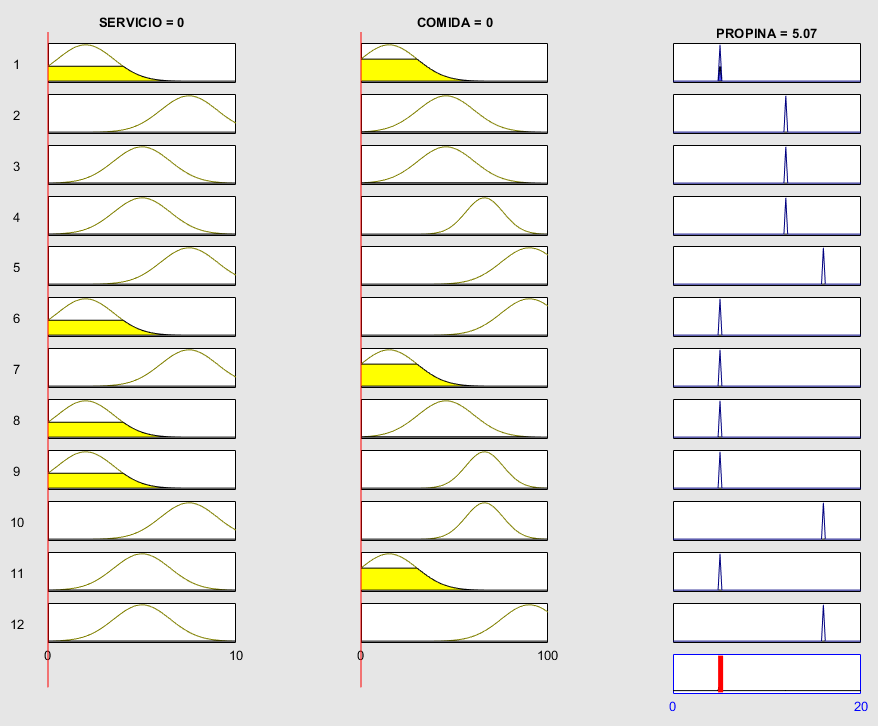
\includegraphics[width=1.4\textwidth]{IMG/RP11.png}
		\label{fig:G3}
	\end{subfigure}
	\hfill
	\begin{subfigure}{0.42\textwidth} % Reducido de 0.45
		\centering
		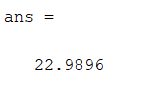
\includegraphics[width=0.8\textwidth]{IMG/M11.png}
		\label{fig:G4}
	\end{subfigure}
	\label{fig:comparacion2}
\end{figure}

A la izquierda se muestran los resultados del toolbox y a la derecha el resultado del sistema programado paso a paso. 
Fuzzy toolbox reporta un valor de 24.4 para el caso planteado, mientras que el sistema programado paso a paso muestra un valor de 22.99. La diferencia entre ambos casos es resulta llamativa, puesto que difieren en más de una unidad ambos resultados con los mismos parámetros pero para efectos prácticos, es aceptable. Jugabilidad de 0, Gráficos de 0 y una historia de 0 llegan a dar como resultado una Calificación de 24.4 (Pésimo).

\newpage

\subsubsection{Caso medio}
Para el caso mínimo, se propone  $JUGABILIDAD = 50$, $GRÁFICOS = 50$ y $HISTORIA = 50$ para ver como se comportan ambas versiones ante la situación intermedia.

\begin{figure}[h]
	\centering
	\begin{subfigure}{0.40\textwidth} % Reducido de 0.45
		\centering
		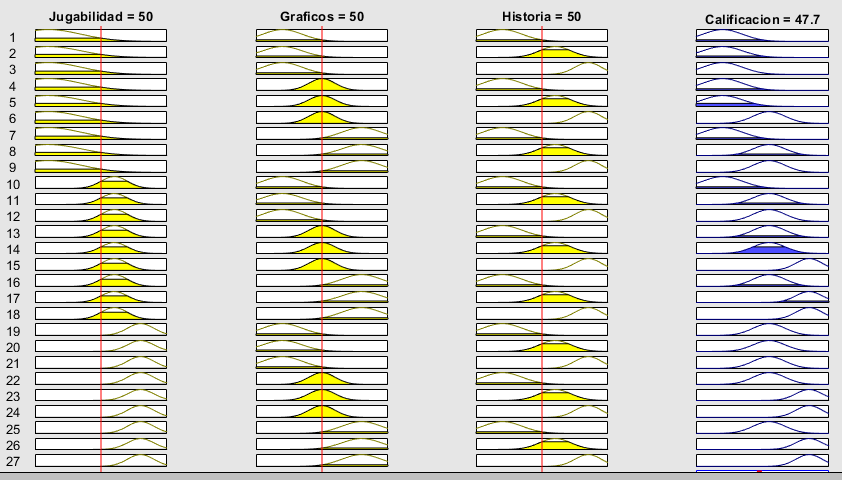
\includegraphics[width=1.4\textwidth]{IMG/RP12.png}
		\label{fig:G5}
	\end{subfigure}
	\hfill
	\begin{subfigure}{0.42\textwidth} % Reducido de 0.45
		\centering
		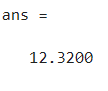
\includegraphics[width=0.8\textwidth]{IMG/M12.png}
		\label{fig:G6}
	\end{subfigure}
	\label{fig:comparacion3}
\end{figure}

A la izquierda se muestran los resultados del toolbox y a la derecha el resultado del sistema programado paso a paso. 
Fuzzy toolbox reporta un valor de 47.7 para el caso planteado, mientras que el sistema programado paso a paso muestra un valor de 52.66. La diferencia entre ambos casos es resulta llamativa, puesto que difieren en más de 4 unidades, ambos resultados con los mismos parámetros pero para efectos prácticos, es aceptable. Jugabilidad de 50, Gráficos de 50 y una historia de 50 llegan a dar como resultado una Calificación de 47.7 (Pasable).

\newpage

\subsubsection{Caso máximo}
Para el caso máximo, se propone  $JUGABILIDAD = 100$, $GRÁFICOS = 100$ y $HISTORIA = 100$ para ver como se comportan ambas versiones ante la situación extrema de puntuar todo al máximo.

\begin{figure}[h]
	\centering
	\begin{subfigure}{0.40\textwidth} % Reducido de 0.45
		\centering
		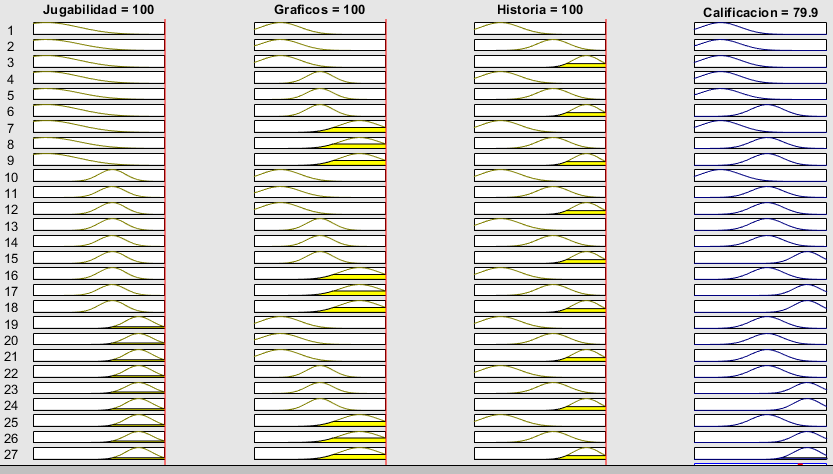
\includegraphics[width=1.4\textwidth]{IMG/RP13.png}
		\label{fig:G7}
	\end{subfigure}
	\hfill
	\begin{subfigure}{0.42\textwidth} % Reducido de 0.45
		\centering
		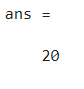
\includegraphics[width=0.8\textwidth]{IMG/M13.png}
		\label{fig:G8}
	\end{subfigure}
	\label{fig:comparacion4}
\end{figure}

A la izquierda se muestran los resultados del toolbox y a la derecha el resultado del sistema programado paso a paso. 
Fuzzy toolbox reporta un valor de 79.9 para el caso planteado, mientras que el sistema programado paso a paso muestra un valor de 83.61. La diferencia entre ambos casos es resulta llamativa, puesto que difieren en más de 3 unidades, ambos resultados con los mismos parámetros pero para efectos prácticos, es aceptable. Jugabilidad de 100, Gráficos de 100 y una historia de 100 llegan a dar como resultado una Calificación de 79.9 (Alta).


\newpage

\section{Conclusiones}

Tras la implementación del problema con 3 variables, cabe mencionar como la adición de las variables y las reglas al código de vuelve sistemático y un poco repetitivo, sin embargo, Es evidente que debe hacerse con paciencia y cuidado para la implementación de las reglas, puesto que la base de reglas aumenta y con ello también los cálculos que son requeridos. Esto se puede notar en la diferencia notable de más de una unidad que existe entre la implementación propuesta y el Fuzzy Logic. 

También cabe recalcar sobre la importancia de entender el problema porque al aumentar el numero de variables que se esta manejando, aumenta consigo la complejidad del mismo, al punto que ya no se puede visualizar tan fácil la gráfica de superficie como indicativo de que tan bien va quedando la modelación.



\newpage

\section{Referencias}

\bibliographystyle{apalike}  % Estilo de cita, puedes cambiarlo si lo prefieres.
\bibliography{Biblio}         % Aquí incluyes el archivo .bib (sin extensión).

\newpage

\section{Anexos}

Este reporte se envía con los códigos anexos que corresponden a:

\begin{enumerate}
	\item Archivo .fiz del sistema difuso para el problema de la calificación con la desfuzificación.
	\item Código en matlab para ejecutar el sistema difuso programado para el problema de la calificación.

\end{enumerate}



\end{document}

